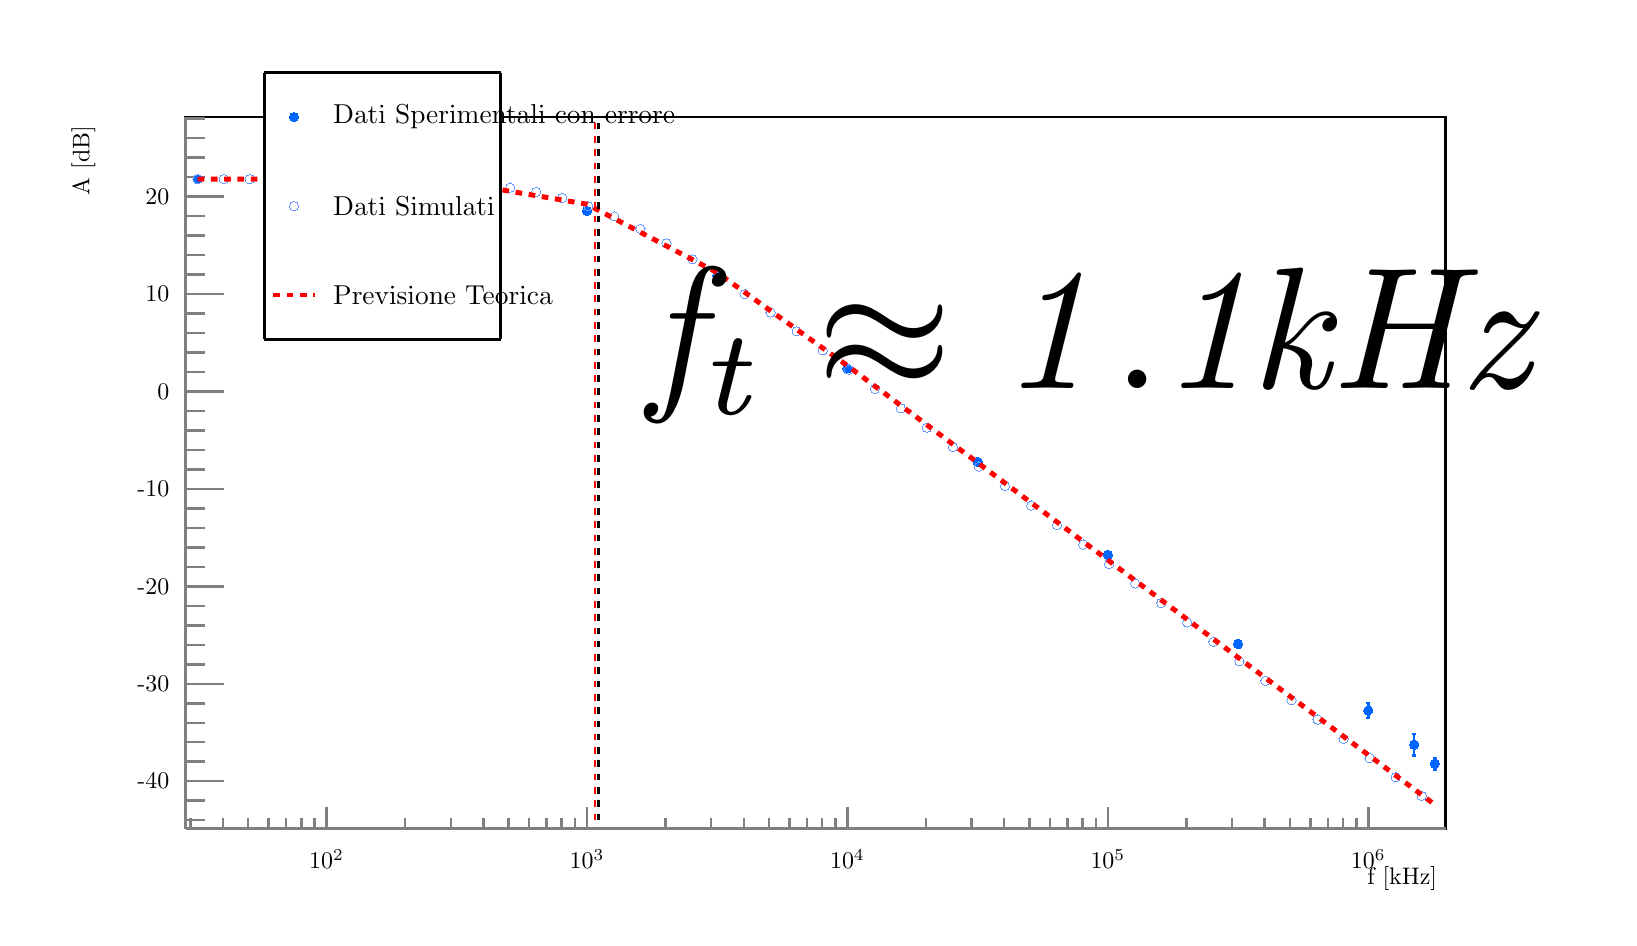
\begin{tikzpicture}
\pgfdeclareplotmark{cross} {
\pgfpathmoveto{\pgfpoint{-0.3\pgfplotmarksize}{\pgfplotmarksize}}
\pgfpathlineto{\pgfpoint{+0.3\pgfplotmarksize}{\pgfplotmarksize}}
\pgfpathlineto{\pgfpoint{+0.3\pgfplotmarksize}{0.3\pgfplotmarksize}}
\pgfpathlineto{\pgfpoint{+1\pgfplotmarksize}{0.3\pgfplotmarksize}}
\pgfpathlineto{\pgfpoint{+1\pgfplotmarksize}{-0.3\pgfplotmarksize}}
\pgfpathlineto{\pgfpoint{+0.3\pgfplotmarksize}{-0.3\pgfplotmarksize}}
\pgfpathlineto{\pgfpoint{+0.3\pgfplotmarksize}{-1.\pgfplotmarksize}}
\pgfpathlineto{\pgfpoint{-0.3\pgfplotmarksize}{-1.\pgfplotmarksize}}
\pgfpathlineto{\pgfpoint{-0.3\pgfplotmarksize}{-0.3\pgfplotmarksize}}
\pgfpathlineto{\pgfpoint{-1.\pgfplotmarksize}{-0.3\pgfplotmarksize}}
\pgfpathlineto{\pgfpoint{-1.\pgfplotmarksize}{0.3\pgfplotmarksize}}
\pgfpathlineto{\pgfpoint{-0.3\pgfplotmarksize}{0.3\pgfplotmarksize}}
\pgfpathclose
\pgfusepathqstroke
}
\pgfdeclareplotmark{cross*} {
\pgfpathmoveto{\pgfpoint{-0.3\pgfplotmarksize}{\pgfplotmarksize}}
\pgfpathlineto{\pgfpoint{+0.3\pgfplotmarksize}{\pgfplotmarksize}}
\pgfpathlineto{\pgfpoint{+0.3\pgfplotmarksize}{0.3\pgfplotmarksize}}
\pgfpathlineto{\pgfpoint{+1\pgfplotmarksize}{0.3\pgfplotmarksize}}
\pgfpathlineto{\pgfpoint{+1\pgfplotmarksize}{-0.3\pgfplotmarksize}}
\pgfpathlineto{\pgfpoint{+0.3\pgfplotmarksize}{-0.3\pgfplotmarksize}}
\pgfpathlineto{\pgfpoint{+0.3\pgfplotmarksize}{-1.\pgfplotmarksize}}
\pgfpathlineto{\pgfpoint{-0.3\pgfplotmarksize}{-1.\pgfplotmarksize}}
\pgfpathlineto{\pgfpoint{-0.3\pgfplotmarksize}{-0.3\pgfplotmarksize}}
\pgfpathlineto{\pgfpoint{-1.\pgfplotmarksize}{-0.3\pgfplotmarksize}}
\pgfpathlineto{\pgfpoint{-1.\pgfplotmarksize}{0.3\pgfplotmarksize}}
\pgfpathlineto{\pgfpoint{-0.3\pgfplotmarksize}{0.3\pgfplotmarksize}}
\pgfpathclose
\pgfusepathqfillstroke
}
\pgfdeclareplotmark{newstar} {
\pgfpathmoveto{\pgfqpoint{0pt}{\pgfplotmarksize}}
\pgfpathlineto{\pgfqpointpolar{44}{0.5\pgfplotmarksize}}
\pgfpathlineto{\pgfqpointpolar{18}{\pgfplotmarksize}}
\pgfpathlineto{\pgfqpointpolar{-20}{0.5\pgfplotmarksize}}
\pgfpathlineto{\pgfqpointpolar{-54}{\pgfplotmarksize}}
\pgfpathlineto{\pgfqpointpolar{-90}{0.5\pgfplotmarksize}}
\pgfpathlineto{\pgfqpointpolar{234}{\pgfplotmarksize}}
\pgfpathlineto{\pgfqpointpolar{198}{0.5\pgfplotmarksize}}
\pgfpathlineto{\pgfqpointpolar{162}{\pgfplotmarksize}}
\pgfpathlineto{\pgfqpointpolar{134}{0.5\pgfplotmarksize}}
\pgfpathclose
\pgfusepathqstroke
}
\pgfdeclareplotmark{newstar*} {
\pgfpathmoveto{\pgfqpoint{0pt}{\pgfplotmarksize}}
\pgfpathlineto{\pgfqpointpolar{44}{0.5\pgfplotmarksize}}
\pgfpathlineto{\pgfqpointpolar{18}{\pgfplotmarksize}}
\pgfpathlineto{\pgfqpointpolar{-20}{0.5\pgfplotmarksize}}
\pgfpathlineto{\pgfqpointpolar{-54}{\pgfplotmarksize}}
\pgfpathlineto{\pgfqpointpolar{-90}{0.5\pgfplotmarksize}}
\pgfpathlineto{\pgfqpointpolar{234}{\pgfplotmarksize}}
\pgfpathlineto{\pgfqpointpolar{198}{0.5\pgfplotmarksize}}
\pgfpathlineto{\pgfqpointpolar{162}{\pgfplotmarksize}}
\pgfpathlineto{\pgfqpointpolar{134}{0.5\pgfplotmarksize}}
\pgfpathclose
\pgfusepathqfillstroke
}
\definecolor{c}{rgb}{1,1,1};
\draw [color=c, fill=c] (0,0) rectangle (20,11.2935);
\draw [color=c, fill=c] (2,1.12935) rectangle (18,10.1641);
\definecolor{c}{rgb}{0,0,0};
\draw [c,line width=0.9] (2,1.12935) -- (2,10.1641) -- (18,10.1641) -- (18,1.12935) -- (2,1.12935);
\definecolor{c}{rgb}{1,1,1};
\draw [color=c, fill=c] (2,1.12935) rectangle (18,10.1641);
\definecolor{c}{rgb}{0,0,0};
\draw [c,line width=0.9] (2,1.12935) -- (2,10.1641) -- (18,10.1641) -- (18,1.12935) -- (2,1.12935);
\definecolor{c}{rgb}{0.5,0.5,0.5};
\draw [c,line width=0.9] (2,1.12935) -- (18,1.12935);
\draw [c,line width=0.9] (2.05864,1.26487) -- (2.05864,1.12935);
\draw [c,line width=0.9] (2.47189,1.26487) -- (2.47189,1.12935);
\draw [c,line width=0.9] (2.79244,1.26487) -- (2.79244,1.12935);
\draw [c,line width=0.9] (3.05434,1.26487) -- (3.05434,1.12935);
\draw [c,line width=0.9] (3.27578,1.26487) -- (3.27578,1.12935);
\draw [c,line width=0.9] (3.46759,1.26487) -- (3.46759,1.12935);
\draw [c,line width=0.9] (3.63679,1.26487) -- (3.63679,1.12935);
\draw [c,line width=0.9] (3.78814,1.40039) -- (3.78814,1.12935);
\definecolor{c}{rgb}{0,0,0};
\draw [anchor=base] (3.78814,0.618317) node[scale=0.864912, color=c, rotate=0]{$10^{2}$};
\definecolor{c}{rgb}{0.5,0.5,0.5};
\draw [c,line width=0.9] (4.78384,1.26487) -- (4.78384,1.12935);
\draw [c,line width=0.9] (5.36629,1.26487) -- (5.36629,1.12935);
\draw [c,line width=0.9] (5.77954,1.26487) -- (5.77954,1.12935);
\draw [c,line width=0.9] (6.10009,1.26487) -- (6.10009,1.12935);
\draw [c,line width=0.9] (6.36199,1.26487) -- (6.36199,1.12935);
\draw [c,line width=0.9] (6.58343,1.26487) -- (6.58343,1.12935);
\draw [c,line width=0.9] (6.77524,1.26487) -- (6.77524,1.12935);
\draw [c,line width=0.9] (6.94444,1.26487) -- (6.94444,1.12935);
\draw [c,line width=0.9] (7.09579,1.40039) -- (7.09579,1.12935);
\definecolor{c}{rgb}{0,0,0};
\draw [anchor=base] (7.09579,0.618317) node[scale=0.864912, color=c, rotate=0]{$10^{3}$};
\definecolor{c}{rgb}{0.5,0.5,0.5};
\draw [c,line width=0.9] (8.09149,1.26487) -- (8.09149,1.12935);
\draw [c,line width=0.9] (8.67394,1.26487) -- (8.67394,1.12935);
\draw [c,line width=0.9] (9.08719,1.26487) -- (9.08719,1.12935);
\draw [c,line width=0.9] (9.40774,1.26487) -- (9.40774,1.12935);
\draw [c,line width=0.9] (9.66964,1.26487) -- (9.66964,1.12935);
\draw [c,line width=0.9] (9.89108,1.26487) -- (9.89108,1.12935);
\draw [c,line width=0.9] (10.0829,1.26487) -- (10.0829,1.12935);
\draw [c,line width=0.9] (10.2521,1.26487) -- (10.2521,1.12935);
\draw [c,line width=0.9] (10.4034,1.40039) -- (10.4034,1.12935);
\definecolor{c}{rgb}{0,0,0};
\draw [anchor=base] (10.4034,0.618317) node[scale=0.864912, color=c, rotate=0]{$10^{4}$};
\definecolor{c}{rgb}{0.5,0.5,0.5};
\draw [c,line width=0.9] (11.3991,1.26487) -- (11.3991,1.12935);
\draw [c,line width=0.9] (11.9816,1.26487) -- (11.9816,1.12935);
\draw [c,line width=0.9] (12.3948,1.26487) -- (12.3948,1.12935);
\draw [c,line width=0.9] (12.7154,1.26487) -- (12.7154,1.12935);
\draw [c,line width=0.9] (12.9773,1.26487) -- (12.9773,1.12935);
\draw [c,line width=0.9] (13.1987,1.26487) -- (13.1987,1.12935);
\draw [c,line width=0.9] (13.3905,1.26487) -- (13.3905,1.12935);
\draw [c,line width=0.9] (13.5597,1.26487) -- (13.5597,1.12935);
\draw [c,line width=0.9] (13.7111,1.40039) -- (13.7111,1.12935);
\definecolor{c}{rgb}{0,0,0};
\draw [anchor=base] (13.7111,0.618317) node[scale=0.864912, color=c, rotate=0]{$10^{5}$};
\definecolor{c}{rgb}{0.5,0.5,0.5};
\draw [c,line width=0.9] (14.7068,1.26487) -- (14.7068,1.12935);
\draw [c,line width=0.9] (15.2892,1.26487) -- (15.2892,1.12935);
\draw [c,line width=0.9] (15.7025,1.26487) -- (15.7025,1.12935);
\draw [c,line width=0.9] (16.023,1.26487) -- (16.023,1.12935);
\draw [c,line width=0.9] (16.2849,1.26487) -- (16.2849,1.12935);
\draw [c,line width=0.9] (16.5064,1.26487) -- (16.5064,1.12935);
\draw [c,line width=0.9] (16.6982,1.26487) -- (16.6982,1.12935);
\draw [c,line width=0.9] (16.8674,1.26487) -- (16.8674,1.12935);
\draw [c,line width=0.9] (17.0187,1.40039) -- (17.0187,1.12935);
\definecolor{c}{rgb}{0,0,0};
\draw [anchor=base] (17.0187,0.618317) node[scale=0.864912, color=c, rotate=0]{$10^{6}$};
\draw [anchor= east] (18,0.496912) node[scale=0.864912, color=c, rotate=0]{f [kHz]};
\definecolor{c}{rgb}{0.5,0.5,0.5};
\draw [c,line width=0.9] (2,1.12935) -- (2,10.1641);
\draw [c,line width=0.9] (2.48,1.73061) -- (2,1.73061);
\draw [c,line width=0.9] (2.24,1.9781) -- (2,1.9781);
\draw [c,line width=0.9] (2.24,2.22558) -- (2,2.22558);
\draw [c,line width=0.9] (2.24,2.47306) -- (2,2.47306);
\draw [c,line width=0.9] (2.24,2.72055) -- (2,2.72055);
\draw [c,line width=0.9] (2.48,2.96803) -- (2,2.96803);
\draw [c,line width=0.9] (2.24,3.21551) -- (2,3.21551);
\draw [c,line width=0.9] (2.24,3.46299) -- (2,3.46299);
\draw [c,line width=0.9] (2.24,3.71048) -- (2,3.71048);
\draw [c,line width=0.9] (2.24,3.95796) -- (2,3.95796);
\draw [c,line width=0.9] (2.48,4.20544) -- (2,4.20544);
\draw [c,line width=0.9] (2.24,4.45293) -- (2,4.45293);
\draw [c,line width=0.9] (2.24,4.70041) -- (2,4.70041);
\draw [c,line width=0.9] (2.24,4.94789) -- (2,4.94789);
\draw [c,line width=0.9] (2.24,5.19538) -- (2,5.19538);
\draw [c,line width=0.9] (2.48,5.44286) -- (2,5.44286);
\draw [c,line width=0.9] (2.24,5.69034) -- (2,5.69034);
\draw [c,line width=0.9] (2.24,5.93782) -- (2,5.93782);
\draw [c,line width=0.9] (2.24,6.18531) -- (2,6.18531);
\draw [c,line width=0.9] (2.24,6.43279) -- (2,6.43279);
\draw [c,line width=0.9] (2.48,6.68027) -- (2,6.68027);
\draw [c,line width=0.9] (2.24,6.92776) -- (2,6.92776);
\draw [c,line width=0.9] (2.24,7.17524) -- (2,7.17524);
\draw [c,line width=0.9] (2.24,7.42272) -- (2,7.42272);
\draw [c,line width=0.9] (2.24,7.6702) -- (2,7.6702);
\draw [c,line width=0.9] (2.48,7.91769) -- (2,7.91769);
\draw [c,line width=0.9] (2.24,8.16517) -- (2,8.16517);
\draw [c,line width=0.9] (2.24,8.41265) -- (2,8.41265);
\draw [c,line width=0.9] (2.24,8.66014) -- (2,8.66014);
\draw [c,line width=0.9] (2.24,8.90762) -- (2,8.90762);
\draw [c,line width=0.9] (2.48,9.1551) -- (2,9.1551);
\draw [c,line width=0.9] (2.48,1.73061) -- (2,1.73061);
\draw [c,line width=0.9] (2.24,1.48313) -- (2,1.48313);
\draw [c,line width=0.9] (2.24,1.23565) -- (2,1.23565);
\draw [c,line width=0.9] (2.48,9.1551) -- (2,9.1551);
\draw [c,line width=0.9] (2.24,9.40259) -- (2,9.40259);
\draw [c,line width=0.9] (2.24,9.65007) -- (2,9.65007);
\draw [c,line width=0.9] (2.24,9.89755) -- (2,9.89755);
\draw [c,line width=0.9] (2.24,10.145) -- (2,10.145);
\definecolor{c}{rgb}{0,0,0};
\draw [anchor= east] (1.9,1.73061) node[scale=0.864912, color=c, rotate=0]{-40};
\draw [anchor= east] (1.9,2.96803) node[scale=0.864912, color=c, rotate=0]{-30};
\draw [anchor= east] (1.9,4.20544) node[scale=0.864912, color=c, rotate=0]{-20};
\draw [anchor= east] (1.9,5.44286) node[scale=0.864912, color=c, rotate=0]{-10};
\draw [anchor= east] (1.9,6.68027) node[scale=0.864912, color=c, rotate=0]{0};
\draw [anchor= east] (1.9,7.91769) node[scale=0.864912, color=c, rotate=0]{10};
\draw [anchor= east] (1.9,9.1551) node[scale=0.864912, color=c, rotate=0]{20};
\draw [anchor= east] (0.701947,10.1641) node[scale=0.864912, color=c, rotate=90]{A [dB]};
\definecolor{c}{rgb}{0,0.4,1};
\foreach \P in {(2.15135,9.37827), (3.78814,9.3578), (5.44093,9.32368), (7.09579,8.97445), (8.74949,8.1498), (10.4034,6.97158), (12.0573,5.78632), (13.7111,4.60553), (15.3649,3.47083), (17.0187,2.62942), (17.6012,2.19362),
 (17.8631,1.95379)}{\draw[mark options={color=c,fill=c},mark size=1.681682pt, line width=0.000000pt, mark=*] plot coordinates {\P};}
\draw [c,line width=0.9] (2.15135,9.40609) -- (2.15135,9.41122);
\draw [c,line width=0.9] (2.12353,9.41122) -- (2.17917,9.41122);
\draw [c,line width=0.9] (2.15135,9.35046) -- (2.15135,9.34533);
\draw [c,line width=0.9] (2.12353,9.34533) -- (2.17917,9.34533);
\draw [c,line width=0.9] (3.78814,9.38562) -- (3.78814,9.39049);
\draw [c,line width=0.9] (3.76032,9.39049) -- (3.81596,9.39049);
\draw [c,line width=0.9] (3.78814,9.32998) -- (3.78814,9.32511);
\draw [c,line width=0.9] (3.76032,9.32511) -- (3.81596,9.32511);
\draw [c,line width=0.9] (5.44093,9.35149) -- (5.44093,9.35666);
\draw [c,line width=0.9] (5.41311,9.35666) -- (5.46875,9.35666);
\draw [c,line width=0.9] (5.44093,9.29586) -- (5.44093,9.29069);
\draw [c,line width=0.9] (5.41311,9.29069) -- (5.46875,9.29069);
\draw [c,line width=0.9] (8.74949,8.17761) -- (8.74949,8.17912);
\draw [c,line width=0.9] (8.72167,8.17912) -- (8.7773,8.17912);
\draw [c,line width=0.9] (8.74949,8.12198) -- (8.74949,8.12047);
\draw [c,line width=0.9] (8.72167,8.12047) -- (8.7773,8.12047);
\draw [c,line width=0.9] (15.3649,3.49865) -- (15.3649,3.51773);
\draw [c,line width=0.9] (15.3371,3.51773) -- (15.3927,3.51773);
\draw [c,line width=0.9] (15.3649,3.44301) -- (15.3649,3.42393);
\draw [c,line width=0.9] (15.3371,3.42393) -- (15.3927,3.42393);
\draw [c,line width=0.9] (17.0187,2.65723) -- (17.0187,2.72309);
\draw [c,line width=0.9] (16.9909,2.72309) -- (17.0466,2.72309);
\draw [c,line width=0.9] (17.0187,2.6016) -- (17.0187,2.53575);
\draw [c,line width=0.9] (16.9909,2.53575) -- (17.0466,2.53575);
\draw [c,line width=0.9] (17.6012,2.22144) -- (17.6012,2.33226);
\draw [c,line width=0.9] (17.5734,2.33226) -- (17.629,2.33226);
\draw [c,line width=0.9] (17.6012,2.16581) -- (17.6012,2.05499);
\draw [c,line width=0.9] (17.5734,2.05499) -- (17.629,2.05499);
\draw [c,line width=0.9] (17.8631,1.9816) -- (17.8631,2.02533);
\draw [c,line width=0.9] (17.8353,2.02533) -- (17.8909,2.02533);
\draw [c,line width=0.9] (17.8631,1.92597) -- (17.8631,1.88224);
\draw [c,line width=0.9] (17.8353,1.88224) -- (17.8909,1.88224);
\definecolor{c}{rgb}{0.4,0.6,1};
\foreach \P in {(2.15135,9.37835), (2.48211,9.37807), (2.81288,9.37763), (3.14364,9.37692), (3.47441,9.37581), (3.80517,9.37405), (4.13594,9.37127), (4.4667,9.3669), (4.79747,9.36005), (5.12823,9.34935), (5.459,9.33284), (5.78976,9.30765),
 (6.12053,9.27001), (6.45129,9.21527), (6.78206,9.13855), (7.11282,9.03572), (7.44359,8.90473), (7.77435,8.74632), (8.10512,8.56373), (8.43588,8.36162), (8.76665,8.14488), (9.09741,7.91774), (9.42818,7.6835), (9.75894,7.44454), (10.0897,7.20251),
 (10.4205,6.95849), (10.7512,6.71321), (11.082,6.46712), (11.4128,6.22052), (11.7435,5.9736), (12.0743,5.72647), (12.4051,5.47921), (12.7358,5.23188), (13.0666,4.9845), (13.3974,4.73709), (13.7281,4.48968), (14.0589,4.24228), (14.3897,3.99491),
 (14.7204,3.74758), (15.0512,3.50033), (15.3819,3.25322), (15.7127,3.00633), (16.0435,2.75977), (16.3742,2.51376), (16.705,2.2686), (17.0358,2.0248), (17.3665,1.78314), (17.6973,1.54485)}{\draw[mark options={color=c,fill=c},mark size=1.681682pt, line
 width=0.000000pt, mark=o] plot coordinates {\P};}
\definecolor{c}{rgb}{1,0,0};
\draw [c,dash pattern=on 2.40pt off 2.40pt ,line width=1.8] (2.15135,9.37824) -- (3.78814,9.37433) -- (5.44093,9.33668) -- (7.09579,9.05857) -- (8.74949,8.18953) -- (10.4034,7.00773) -- (12.0573,5.7762) -- (13.7111,4.53939) -- (15.3649,3.30203) --
 (17.0187,2.06463) -- (17.6012,1.62883) -- (17.8631,1.43287);
\definecolor{c}{rgb}{0,0,0};
\draw [c,dash pattern=on 2.40pt off 2.40pt ,line width=0.9] (7.24338,1.23565) -- (7.24338,10.145);
\definecolor{c}{rgb}{1,0,0};
\draw [c,dash pattern=on 2.40pt off 2.40pt ,line width=0.9] (7.19574,1.23565) -- (7.19574,10.145);
\definecolor{c}{rgb}{0,0,0};
\draw [anchor=north west] (7.09579,9.03136) node[scale=6.27061, color=c, rotate=0]{$\it{f_{t}}\approx 1.1 kHz$};
\definecolor{c}{rgb}{1,1,1};
\draw [color=c, fill=c] (3,7.34075) rectangle (6,10.7288);
\definecolor{c}{rgb}{0,0,0};
\draw [c,line width=0.9] (3,7.34075) -- (6,7.34075);
\draw [c,line width=0.9] (6,7.34075) -- (6,10.7288);
\draw [c,line width=0.9] (6,10.7288) -- (3,10.7288);
\draw [c,line width=0.9] (3,10.7288) -- (3,7.34075);
\draw [anchor= west] (3.75,10.1641) node[scale=0.988471, color=c, rotate=0]{Dati Sperimentali con errore};
\definecolor{c}{rgb}{0,0.4,1};
\foreach \P in {(3.375,10.1641)}{\draw[mark options={color=c,fill=c},mark size=1.681682pt, line width=0.000000pt, mark=*] plot coordinates {\P};}
\definecolor{c}{rgb}{0,0,0};
\draw [anchor= west] (3.75,9.03477) node[scale=0.988471, color=c, rotate=0]{Dati Simulati};
\definecolor{c}{rgb}{0.4,0.6,1};
\foreach \P in {(3.375,9.03477)}{\draw[mark options={color=c,fill=c},mark size=1.681682pt, line width=0.000000pt, mark=o] plot coordinates {\P};}
\definecolor{c}{rgb}{0,0,0};
\draw [anchor= west] (3.75,7.90542) node[scale=0.988471, color=c, rotate=0]{Previsione Teorica};
\definecolor{c}{rgb}{1,0,0};
\draw [c,dash pattern=on 2.40pt off 2.40pt ,line width=1.8] (3.1125,7.90542) -- (3.6375,7.90542);
\end{tikzpicture}
